\documentclass[
	a4paper,%
	notoc,%
	nobib,%
	nols,%
	nofonts,%
	% marginals=raggedouter,%
	% symmetric%
	]{tufte-book} % Use the tufte-book class which in turn uses the tufte-common class
\hypersetup{colorlinks=false,
			linktocpage,
			% pdfborder={0 0 1},
} % Comment this line if you don't wish to have colored links

\makeatletter
\renewcommand*\l@figure{\@dottedtocline{1}{1.5em}{2.3em}}
\makeatother

\usepackage{microtype} % Improves character and word spacing
% \usepackage{zhmCJK}
% \setCJKmainfont{fonts/FandolSong-Regular.ttf}[
	% BoldFont = fonts/FandolSong-Bold.ttf,
	% ItalicFont = fonts/FandolKai-Regular.ttf
% ]
\usepackage{xeCJK}
\setCJKmainfont{Source Han Serif SC}[
	BoldFont = Source Han Serif SC Bold,
	ItalicFont = FZNewKai-Z03
]
\setmonofont{Bitstream Vera Sans Mono}[Scale=MatchLowercase]
\usepackage{fontspec}
% \usepackage{polyglossia}
% \usepackage[nonoverlap]{ruby}
% \renewcommand\rubysize{0.6}
\renewcommand\smallcaps[1]{%
	{\addfontfeature{LetterSpace=5.0}\textsc{\MakeLowercase{#1}}}}

\setmainfont{Garamond Premier Pro}[
  Numbers=OldStyle,
  ItalicFont=Garamond Premier Pro Italic,
  % ItalicFeatures={
  % SizeFeatures={
	  % {Size={12-}, Ligatures={Common, Rare}}
  % }},
  Ligatures={Common},
]%%
\newfontfamily\headingfont[
  Ligatures={Common,Rare,Historic},
  ItalicFont=Garamond Premier Pro Italic Display,
  Numbers=OldStyle,
]{Garamond Premier Pro Display}
\newfontfamily\fancyfont[
  Ligatures={Common,Rare,Historic},
  ItalicFont=Garamond Premier Pro Italic,
  Numbers=OldStyle,
]{Garamond Premier Pro}
\newfontfamily\secfont[
  % Ligatures={Common,Rare,Historic},
  ItalicFont=Garamond Premier Pro Semibold Italic Caption,
  Numbers=OldStyle,
]{Garamond Premier Pro Semibold Caption}

% \newlength\TitleOverhang
% \setlength\TitleOverhang{.6cm}

% \newcommand\Overhang[1]{%
  % \llap{\makebox[\TitleOverhang][l]{#1}}%
% }
% \titleformat{\section}
  % {\fancyfont\Large\itshape}{\Overhang\thesection}{0em}{}
\usepackage[inline]{enumitem}
\usepackage{xpinyin}
% \setitemize{noitemsep,topsep=0pt,parsep=0pt,partopsep=0pt}
\setlist{noitemsep,topsep=0pt,parsep=0pt,partopsep=0pt}
\usepackage[parfill]{parskip}
% \setlength{\parindent}{0px}
\makeatletter
% Paragraph indentation and separation for normal text
\renewcommand{\@tufte@reset@par}{%
  \setlength{\RaggedRightParindent}{0.0pc}%
  \setlength{\JustifyingParindent}{0.0pc}%
  \setlength{\parindent}{0pc}%
  \setlength{\parskip}{\baselineskip}%
}
\@tufte@reset@par
\makeatother

\makeatletter
\newcommand\chapterauthor[1]{#1\gdef\@chapterauthor{#1}}
\def\@chapterauthor{}
\fancypagestyle{mystyle}{%
\fancyhf{}%
\renewcommand{\chaptermark}[1]{\markboth{##1}{}}%
\fancyhead[LE]{\thepage\quad\smallcaps{\newlinetospace{\leftmark}}}%
\fancyhead[RO]{\smallcaps{\newlinetospace{\@chapterauthor}}\quad\thepage}%
}
\makeatother

% \usepackage[T1]{fontenc}
% \usepackage[utf8]{inputenc}
\usepackage[greek,russian,english]{babel}

\usepackage{expex}
\makeatletter
\renewcommand{\exnoprint}{\llap{\ep@exnoformat{\ep@rawexnoprint}}}
\makeatother
\usepackage{titletoc,mdframed,pdfpages,soul,varioref,pgfplots}
\usepackage[acronym]{glossaries}
\pgfplotsset{
compat=newest,
ticklabel style = {font=\footnotesize},
grid style={dotted,black},
}
\usetikzlibrary{pgfplots.dateplot}
\usepgfplotslibrary{dateplot}
  % \usepackage{etoolbox}
  \setcounter{tocdepth}{1}
  \pretocmd{\tableofcontents}{\begin{mdframed}[outermargin=\dimexpr-\marginparwidth-\marginparsep\relax,innermargin=0pt,hidealllines=true]\let\cleardoublepage\relax}{}{}
  \apptocmd{\tableofcontents}{\end{mdframed}}{}{}

\usepackage[backend=bibtex,autocite=footnote,style=authoryear-icomp,natbib=true,dashed=false]{biblatex}

\defbibheading{bibliography}[\bibname]{%
  \chapter*{#1}%
  \markboth{#1}{#1}}

\usepackage{lipsum,lettrine,type1cm} % Inserts dummy text
\newcommand{\dcap}[2]{\lettrine[lines=2, findent=3pt, nindent=0pt]{#1}{}{\smallcaps{#2}}}

\usepackage{booktabs} % Better horizontal rules in tables

\usepackage{graphicx} % Needed to insert images into the document
\graphicspath{{graphics/}} % Sets the default location of pictures
\setkeys{Gin}{width=\linewidth,totalheight=\textheight,keepaspectratio} % Improves figure scaling

\usepackage{fancyvrb} % Allows customization of verbatim environments
\fvset{fontsize=\normalsize} % The font size of all verbatim text can be changed here

\newcommand{\hangp}[1]{\makebox[0pt][r]{(}#1\makebox[0pt][l]{)}} % New command to create parentheses around text in tables which take up no horizontal space - this improves column spacing
\newcommand{\hangstar}{\makebox[0pt][l]{*}} % New command to create asterisks in tables which take up no horizontal space - this improves column spacing

\usepackage{xspace} % Used for printing a trailing space better than using a tilde (~) using the \xspace command

\newcommand{\monthyear}{\ifcase\month\or January\or February\or March\or April\or May\or June\or July\or August\or September\or October\or November\or December\fi\space\number\year} % A command to print the current month and year

\newcommand{\openepigraph}[2]{ % This block sets up a command for printing an epigraph with 2 arguments - the quote and the author
\begin{fullwidth}
\sffamily\large
\begin{doublespace}
\noindent\allcaps{#1}\\ % The quote
\noindent\allcaps{#2} % The author
\end{doublespace}
\end{fullwidth}
}

\newcommand{\blankpage}{\newpage\hbox{}\thispagestyle{empty}\newpage} % Command to insert a blank page

\usepackage{units} % Used for printing standard units

\newcommand{\hlred}[1]{\textcolor{Maroon}{#1}} % Print text in maroon
\newcommand{\hangleft}[1]{\makebox[0pt][r]{#1}} % Used for printing commands in the index, moves the slash left so the command name aligns with the rest of the text in the index
\newcommand{\hairsp}{\hspace{1pt}} % Command to print a very short space
\newcommand{\ie}{\textit{i.\hairsp{}e.}\xspace} % Command to print i.e.
\newcommand{\eg}{\textit{e.\hairsp{}g.}\xspace} % Command to print e.g.
\newcommand{\na}{\quad--} % Used in tables for N/A cells
\newcommand{\measure}[3]{#1/#2$\times$\unit[#3]{pc}} % Typesets the font size, leading, and measure in the form of: 10/12x26 pc.
\newcommand{\tuftebs}{\symbol{'134}} % Command to print a backslash in tt type in OT1/T1

\providecommand{\XeLaTeX}{X\lower.5ex\hbox{\kern-0.15em\reflectbox{E}}\kern-0.1em\LaTeX}
\newcommand{\tXeLaTeX}{\XeLaTeX\index{XeLaTeX@\protect\XeLaTeX}} % Command to print the XeLaTeX logo while simultaneously adding the position to the index

\newcommand{\doccmdnoindex}[2][]{\texttt{\tuftebs#2}} % Command to print a command in texttt with a backslash of tt type without inserting the command into the index

\newcommand{\doccmddef}[2][]{\hlred{\texttt{\tuftebs#2}}\label{cmd:#2}\ifthenelse{\isempty{#1}} % Command to define a command in red and add it to the index
{ % If no package is specified, add the command to the index
\index{#2 command@\protect\hangleft{\texttt{\tuftebs}}\texttt{#2}}% Command name
}
{ % If a package is also specified as a second argument, add the command and package to the index
\index{#2 command@\protect\hangleft{\texttt{\tuftebs}}\texttt{#2} (\texttt{#1} package)}% Command name
\index{#1 package@\texttt{#1} package}\index{packages!#1@\texttt{#1}}% Package name
}}

\newcommand{\doccmd}[2][]{% Command to define a command and add it to the index
\texttt{\tuftebs#2}%
\ifthenelse{\isempty{#1}}% If no package is specified, add the command to the index
{%
\index{#2 command@\protect\hangleft{\texttt{\tuftebs}}\texttt{#2}}% Command name
}
{%
\index{#2 command@\protect\hangleft{\texttt{\tuftebs}}\texttt{#2} (\texttt{#1} package)}% Command name
\index{#1 package@\texttt{#1} package}\index{packages!#1@\texttt{#1}}% Package name
}}

% A bunch of new commands to print commands, arguments, environments, classes, etc within the text using the correct formatting
\newcommand{\docopt}[1]{\ensuremath{\langle}\textrm{\textit{#1}}\ensuremath{\rangle}}
\newcommand{\docarg}[1]{\textrm{\textit{#1}}}
\newenvironment{docspec}{\begin{quotation}\ttfamily\parskip0pt\parindent0pt\ignorespaces}{\end{quotation}}
\newcommand{\docenv}[1]{\texttt{#1}\index{#1 environment@\texttt{#1} environment}\index{environments!#1@\texttt{#1}}}
\newcommand{\docenvdef}[1]{\hlred{\texttt{#1}}\label{env:#1}\index{#1 environment@\texttt{#1} environment}\index{environments!#1@\texttt{#1}}}
\newcommand{\docpkg}[1]{\texttt{#1}\index{#1 package@\texttt{#1} package}\index{packages!#1@\texttt{#1}}}
\newcommand{\doccls}[1]{\texttt{#1}}
\newcommand{\docclsopt}[1]{\texttt{#1}\index{#1 class option@\texttt{#1} class option}\index{class options!#1@\texttt{#1}}}
\newcommand{\docclsoptdef}[1]{\hlred{\texttt{#1}}\label{clsopt:#1}\index{#1 class option@\texttt{#1} class option}\index{class options!#1@\texttt{#1}}}
\newcommand{\docmsg}[2]{\bigskip\begin{fullwidth}\noindent\ttfamily#1\end{fullwidth}\medskip\par\noindent#2}
\newcommand{\docfilehook}[2]{\texttt{#1}\index{file hooks!#2}\index{#1@\texttt{#1}}}
\newcommand{\doccounter}[1]{\texttt{#1}\index{#1 counter@\texttt{#1} counter}}

\usepackage{makeidx} % Used to generate the index
% \makeindex % Generate the index which is printed at the end of the document

\makeatletter
\renewcommand{\@chapapp}{}% Not necessary...
\newenvironment{chapquote}[2][2em]
  {\setlength{\@tempdima}{#1}%
   \def\chapquote@author{#2}%
   \parshape 1 \@tempdima \dimexpr\textwidth-2\@tempdima\relax%
   \itshape}
  {\par\normalfont\hfill---\ \chapquote@author\hspace*{\@tempdima}\par\bigskip}
\makeatother

\newcommand{\cann}{[\smallcaps{can}]}



%----------------------------------------------------------------------------------------
%	BOOK META-INFORMATION
%----------------------------------------------------------------------------------------

\title[Jingran Sheng]{\Large How political argot work as a tool of protesting through border making process and its metaphoric reflection on spacial practice} % Title of the book

\author[Jingran Sheng]{Jingran Sheng} % Author

\publisher{Development Planning Unit, University College London} % Publisher

%----------------------------------------------------------------------------------------

\addbibresource{bibliography.bib} % Use the bibliography.bib file for the bibliography

\newcommand{\ict}{\smallcaps{ict}}
\newcommand{\gfw}{\smallcaps{gfw}}
\newcommand{\oed}{\smallcaps{oed}}
\newcommand{\cpc}{\smallcaps{cpc}}
\newcommand{\prc}{\smallcaps{prc}}
\newcommand{\cnnic}{\smallcaps{cnnic}}
\newcommand{\cernic}{\smallcaps{cernic}}
\newcommand{\cernet}{\smallcaps{cernet}}
\newcommand{\miit}{\smallcaps{miit}}
\newcommand{\mpt}{\smallcaps{mpt}}
\newcommand{\psb}{\smallcaps{psb}}
\newcommand{\isp}{\smallcaps{isp}}
\newcommand{\usa}{\smallcaps{usa}}
\newcommand{\cac}{\smallcaps{cac}}
\newcommand{\mfa}{\smallcaps{mfa}}
\newcommand{\vpn}{\smallcaps{vpn}}
\newcommand{\bbc}{\smallcaps{bbc}}
\newcommand{\uk}{\smallcaps{uk}}

\newcommand{\moha}{\textit{m\'o-h\'a}}
\newcommand{\Moha}{\textit{M\'o-h\'a}}

% \makenoidxglossaries
% \newacronym{ict}{ict}{Information and Communications Technology}
% \newacronym{gfw}{gfw}{Great Firewall of China}
% \newacronym{oed}{oed}{Oxford English Dictionary}
% \newacronym{cpc}{cpc}{Communist Party of China}
% \newacronym{prc}{prc}{People's Republic of China}
% \newacronym{cnnic}{cnnic}{China Internet Network Information Center}
% \newacronym{cernic}{cernic}{China Education and Research Network Information Center}
% \newacronym{cernet}{cernet}{The China Education and Research Network}
% \newacronym{miit}{miit}{Ministry of Industry and Information Technology}
% \newacronym{mpt}{mpt}{Ministry of Posts and Telecommunications of the People's Republic of China}
% \newacronym{psb}{psb}{Public Security Bureau}
% \newacronym{isp}{isp}{Internet Service Provider}
% \newacronym{usa}{usa}{United States of America}
% \newacronym{cau}{cac}{Cyberspace Administration of China}
% \newacronym{mfa}{mfa}{The Ministry of Foreign Affairs of the People's Republic of China}
% \newacronym{vpn}{vpn}{Virtual Private Network}
% \newacronym{bbc}{bbc}{British Broadcasting Corporation}
% \newacronym{uk}{uk}{United Kingdom of Great Britain and Northern Ireland}

\begin{document}

% \maketitle % Print the title page

%----------------------------------------------------------------------------------------
%	COPYRIGHT PAGE
%----------------------------------------------------------------------------------------
\frontmatter
\includepdf{cover3.pdf}
\newpage
% \input{chapters/abstract.tex}
\chapter*{Acknowledgement}

First, I would like to thank my supervisor Giovanna, I could not have made this work possible without her generous guidence and support.

I would also like to thank all the \smallcaps{budd} staff: Camillo Boano, Catalina Ortiz, Giorgio Talocci, Camila Cocina, Ricardo Marten, Kay Pallaris, and Azadeh Mashayekhi, for all the knowledge and inspiration you have given me, and have made this year joyful and valuable; and my classmates, for friendship, ideas, and suggestions.

Special thanks to my friends, Liu Jingyu and Cai Yining for supporting, listening, and giving me suggestions and help for this work; to Lin Qingyuandi, for helping me with technical issues and data collecting.

Finally, I would like to thank my family for your patience, and support for all th choices I have made.

The word count stated on the cover page was produced by the program \TeX count\footnote{\url{http://app.uio.no/ifi/texcount/index.html}} by Einar Andreas Rødland\footnote{\url{http://folk.uio.no/einarro/}}.

Cover illustration: Mabel Tibbitts\footnote{P.~233 in Gibson, Eva Katharine (ca.~1901). \textit{Zauberlinda, the wise witch}. Illustrated by Mabel Tibbitts. Chicago, Lansing: Robt. Smith Printing Co.} (ca.~1901).

\cleardoublepage
\chapter*{Acronyms}

\begin{tabular}[H]{rl}
\smallcaps{bbc} & {British Broadcasting Corporation}\\
\smallcaps{cau} & {Cyberspace Administration of China}\\
\smallcaps{cernet} & {China Education and Research Network}\\
\smallcaps{cernic} & {China Education and Research Network Information Center}\\
\smallcaps{cnnic} & {China Internet Network Information Center}\\
\smallcaps{cpc} & {Communist Party of China}\\
\smallcaps{dns} & {Domain Name Servers}\\
\smallcaps{gfw} & {Great Firewall of China}\\
\smallcaps{ict} & {Information and Communications Technology}\\
\smallcaps{ip} & {Internet Protocol}\\
\smallcaps{isp} & {Internet Service Provider}\\
\smallcaps{mfa} & {Ministry of Foreign Affairs of the People's Republic of China}\\
\smallcaps{miit} & {Ministry of Industry and Information Technology}\\
\smallcaps{mpt} & {Ministry of Posts and Telecommunications of the People's Republic of China}\\
\smallcaps{oed} & {Oxford English Dictionary}\\
\smallcaps{prc} & {People's Republic of China}\\
\smallcaps{psb} & {Public Security Bureau}\\
\smallcaps{uk} & {United Kingdom of Great Britain and Northern Ireland}\\
\smallcaps{usa} & {United States of America}\\
\smallcaps{vpn} & {Virtual Private Network}\\
\end{tabular}

% \begin{fullwidth}
% ~\vfill
% \thispagestyle{empty}
% \end{fullwidth}
% \setcounter{page}{0}\renewcommand{\thepage}{\roman{page}}
\cleardoublepage
\setcounter{tocdepth}{3}
\tableofcontents % Print the table of contents
\begin{fullwidth}
\listoffigures % Print a list of figures
\end{fullwidth}
% \listoftables % Print a list of tables

\cleardoublepage

\mainmatter

\setcounter{secnumdepth}{3}
\setcounter{page}{1} %\renewcommand{\thepage}{\arabic{page}}\pagestyle{plain}
\chapter{Introduction}
\begin{chapquote}[3em]{T.\ S.\ Eliot, \textit{\addfontfeature{ItalicFeatures={Style=Swash}}The Rock}}
	{\fancyfont
		{\addfontfeature{ItalicFeatures={Style=Swash}}Where} is the Life we have lost in living?\\
		\hskip 4.5em Where is the wisdom we have lost in knowledge?\\
		\hskip 3em Where is the knowledge we have lost in information?}
\end{chapquote}

\section{Background}
\dcap{I}{n the summer} of 2016, when Xu Qiuxia, a journalist from Hong Kong, was giving a lecture about journalism to a group of high school students in Beijing, she surprisingly noticed that when she was showing them a 16 years old piece of video footage of the ex-president of China Jiang Zemin, most of the students could recite the whole conversation in the video from their memory. While she didn't know at that time, the same video had been uploaded to the Internet, and already got 1,690,000 views\footnote{Until 15th Aug 2017, there were already 3,019,778 views. The referred video is available at \url{https://youtu.be/lBOwxXxesBo}, was uploaded to YouTube on 3rd Apr 2007.} on YouTube at that time \citep{__2016-2}. The culture phenomena called \moha\ became increasingly popular on Chinese Internet, memes, quotes, and derivatives of Jiang Zemin were created and circulated all over the Internet. Although these memes and their materials have been repeatedly censored and blocked, they have not disappeared, but constantly reappear in more and more abstract and implicit forms.

Building on theories from fields of urban design, politics, and media study, this dissertation intends to build a theoretical framework around two hypotheses. First, space is understood as the medium of political activities, means of surveillance, and the arena where the dominating and subordinate classes maintain or challenge the established social order. While the opportunity of open, organized and direct protest is restricted for lacking economic ability or political power, the subordinate class would tend to use everyday forms of resistance. This entails everyday activities and language occurring in the public space that are creatively hijacked for political purposes to express the discontents and demands of subordinates. Second, the virtual space that is maintained by the Information Communication Technologies (\ict s) could be considered as an extension, in some occasions an alternative of the physical space. The technique of \ict s have several advantages such as synchronicity and decentralization, which provide a chance to create alternative public ``space'', providing new ways of communication and acceleration the existing connections. However, due to complex socio-economical factors in the reality such as language and the economic ability of setting up Internet infrastructure, the social structure and regulative power practiced by the state that exist in the physical space also being extended into the virtual space, with similar logic and mechanism.

This dissertation is intended to consider the virtual space as part of (extended) urban space, which as well as the physical space, plays its roles as the medium of domination and arena of contestation. The culture phenomena of \moha\ that suddenly became popular reflects the rapid change experienced by the country in the early 21st century. This unique case provide an interesting aspect to view the Chinese society, people's reaction to the censorship and surveillance, the subordinate's tactic for political expressions, and the flexibility of language and meme.

\section{Methodology}

Except this chapter of introduction, this dissertation contains two main chapters, followed by a conclusion. Chapter \ref{lit} builds the theoretical framework, based on literatures in the fields of urban design, politics, and media study, two key hypotheses will be discussed and framed: the translations between explicit, direct political expressions and ordinary, implicit ones; and the virtual space as the extension of physical space.

Chapter \ref{case} will be a case study of the subculture of \moha, where I investigated the history of Chinese Internet and relevant policies and regulations, which are the base of the contemporary Internet censorship in China; then, the origin and materials used in the \moha\ subculture---Jiang Zemin's activities, related videos and text materials, etc., will be discussed, followed by a review of the subculture itself, how and by whom the memes relevant contents are being created and circulated. With the theoretical framework established in the previous chapter, the mechanism, and the possible reason and intention behind this subculture will be discussed.

Due to the inaccurate nature of the online information, this dissertation has choosen to use multiple types of sources as research materials. While building the theoretical framework, academic papers and books will be referenced to ensure the theory to be solid and reliable. In the case study, while refer to the censorship and surveillance by the state, original regulations and policies will be cited as they are basis of the government administration. Open source data will be used to analyze the confirmable facts---Internet population, web traffic, etc. For facts related to the \moha\ subculture, because it has never been (nor been allowed to) studied in mainland China, there are limited reliable data sources available, therefore, relatively ``informal'' sources will be used: personal blogs, private news sites, websites with political biases, etc. These sources might include exaggerated information, hearsays, rumours that hard or nearly impossible to verify. Since the focus of this dissertation is on regular Internet users, for whom what information is most widely perceived is not dependent on the reliability, but the accessibility; and they will react on these information assuming they are true; thus these informal information sources will be also important as part of the knowledge of regular Internet users. Therefore, the formal and informal sources will be equally discussed in the case study, while the meta-information of sources will be noted.

\chapter{Theoretical Framework}\label{lit}

\section{Spatial politics and everyday life}

\dcap{I}{n order to} understand the mechanism of protest and other political expressions, it is fundamental to understand the role of space. The term \textit{protest} could be understood as ``any action, act, or statement expressing (emphatic) objection to or dissent from something'' \citep{_protest_2007}. Space, either physical or metaphorical, is where these action, act, or statement take place. The concept of space has became an important component in contemporary literatures and theories of politics and geography.\ %
\marginnote{{``(Social) space is a (social) product. [\ldots] that in addition to being a means of production it is also a means of control, and hence of domination, of power;''} \\\noindent\citep[p.~26]{lefebvre_production_1991}}%
Urban space is understood as not only a physically defined area, but a complicated mix of, as defined by Lefebvre, perceived, conceived, and lived space \citep{schmidt_henry_2008}. Being \textit{in} a city, apart from being inside its geographical border, also means conceiving and picturing the city and the image of the city, and experiencing the everyday life practiced by all residents in the city. The new image and experience thus produced are also fed back to and become part of the city. Space is where human activities take place, while it is also being constantly produced and reproduced by these activities; it creates the political relation between individuals, which brings them together but meanwhile disclose the distinctions between them (\citealp{canovan_politics_1985}, p.~634, cited in \citealp{dikec_space_2012}, p.~672). It has been argued that space is a subject or means of political control, domination, and expression of power. Instead existing as itself, space is contested, and produced by the dynamic of relations. Therefore, it could be argued that space is not political \textit{per se}, but is the ground and medium of political practice, that challenge and reproduce the established order of space through constant contestation \citep{dikec_space_2012,hou_not_2010,henaff_public_2001}.

Politics%
\marginnote{politics, \textit{n}.\\\noindent 2. The theory or practice of government or administration. \citep{_politics_2006}}%
, from its far origin in ancient Greek τὰ πολιτικά (public matters, civic affairs), has been tightly related to the concept of city, from the ancient Greek city-state i.e.\ \textit{polis} (πόλις) to a modern city. \citet[p.~93]{arendt_introduction_2005} argues that politics ``deals with the coexistence and association of \textit{different} men'', that is the fundamental of communal life. Living in a city means an individual obtains freedom by being with others who are marked as equal to them, therefore. The spatial existence of the city not only define the land but also the place where this political freedom is guaranteed. \citeauthor{ranciere_et_2009} (\citeyear{ranciere_et_2009}, cited in \citealt[p.~673]{dikec_space_2012}) argues that politics reconfigures the orders of time and space, hierarchies of places, therefore institutionalised and legitimised forms of domination, which instituted by the form of symbolisation he defined as \textit{police}. Politics in this sense is related to the distribution of space: the function of the space, the right to access the space, etc. Through opening the space, politics then challenges the established order and make new distributions and relations \citep{ranciere_politics_2003}. In terms of governance, which referring to the relations between governor (now usually means the government, or the state) and governed, the central question turns into the process of decision-making: how these decisions are made, what actors are (and are empowered to be) involved in the process, and in whose interest \citep{martin_space_2003}. A more participatory process would allow citizens to be ``deliberately included in the future'' \citep[pp.~216]{arnstein_ladder_1969}, yet this process is also constantly under contestation, as those in power resist to the redistribution of power \citep{arnstein_ladder_1969}. In short, the symbolisation of police institute the order of time and space based on the power relationship between the governed and the governor in the city, this practice of governance then become politics. Space, especially so called public space, which is the medium and ground of the politics, is the arena of political activities that either challenge or maintain the established order.

Public space has long been an important component of cities all over the world but hard to accurately defined. In Burmese,\marginnote{\includegraphics[width=2in]{mmpublic.pdf}\\\noindent``Gathering space'' in Burmese.} there is no has same meaning as what ``public space'' means in Englishg, so the phrase has to be translated to "gathering space". In Chinese,\marginnote{\vskip4mm\noindent{\LARGE 公共空间}\\\vskip2mm\noindent``Public space'' in Chinese.} the word "public" is frequently been understood as ``owned by the state (or an organisation)''. However, what in common is, public spaces are not private, they are not owned by a single individual. In most cities there are places that accessible by the public, in which people are able to gather, socialize, run business, or sometimes protest. These spaces can be square, market, street, park, etc. \citet[p.~35]{henaff_public_2001} define public space as ``simultaneously: open to all, well known by all, and acknowledged by all\ldots\ it stands in opposition to private space of special interests''. Planning as a kind of act, embodies the interntion that power holders tend to shape the planned subject i.e.\ urban space based on their interest. However, public spaces provide the ground for people, citizens, have-nots, to loosen the given order of space and produce opportunities to new ``perceptions, attitudes, and behaviors'' \citep[p.~14]{franck_tying_2006} by challenging or disrupting the intended use of these space, take the space out of the context that has assigned features and nothing unpredictable would happen. These unintended use could be legitimised or not legitimised, impromptu or scheduled, temporary or permanent \citep{franck_tying_2006}. \citet{hou_not_2010} defines the public space that oppose the solely control, regulate, and maintain of state as ``insurgent public space'', the public space can be turned into the ground against the regulation and privatization. According to Maurice Blanchot \citep[cited in][]{sheringham_indeterminacy_2006}, the everyday\footnote{Originally referred as the \textit{quotidien}.} inherently eludes definition, that ``a sector most at the mercy of legislation and bureaucracy was at the same time refractory to such limitation'' \citep[p.~18]{sheringham_indeterminacy_2006}. The everyday life is ``potentially the present, alive with the force of lived but uncategorizable experience'' \citep[p.~17]{sheringham_indeterminacy_2006}. Therefore, it could be argue that the potential that embedded in the practice of everyday life that challenging the order, which established or planned by the power holder. And this process, intended or unintended, by which the power holder is challenged, could be political.


The practice that challenges the established order could occur in varies forms, in fact, it is inexhaustible, something would always remains uncertain, and through which the possibilities of everyday life are maintained \citep{lefebvre_critique_1991}. The massive activity of ``square dancing'' in China is an interesting example\marginnote{``{[O]ne Beijing {\rm yangge} dancer pointed out that ``good health and friends are the most important things in life,'' and that their group dancing is a basic ``{\rm human right}'' that belongs to both natives and visitors of any age in Beijing.''}\\\noindent(\citealp{brownell_training_1995}, cited in \citealp[p.~33]{chen_dancing_2010})}. In cities all over China, peoples, mostly middle-aged or old, gather and dance in the public, with loud, energetic music playing. The group size varies from four to five people to huge groups with more than one hundred people. These groups improvised any available space as the site for dancing, from ordinary public spaces such as squares and parks to road side, building entrances, and parking lots (see figure \vref{fig:squaredance}). This activity became an important element of dancers' life, providing major socializing and maintenance of health for many, with some elder people even use it as a therapy. To support their own practice, their appropriating of the public space ``unintentionally but effectively developing new typologies of hybrid use'' (\citealp{de_certeau_practice_1984}, \citealp[cited in][p.~22]{chen_dancing_2010}) for the spaces designed by urban planners. The square dancing has also been complained a lot, in a few cases, even violent attacked \citep{jacobs_cutting_2015} by residents, usually for making noise and occupying space. In June 2017 during gaokao\footnote{Gaokao is the Chinese annual National Higher Education Entrance Examination, this exam is a prerequisite for all normal student in China mainland to take the undergraduate level education.}, groups of dances in Hunan province collectively decided to stop dance for 10 days, to create a quiet environment for students to prepare for the exam \citep{xinying_squares_2017}. The dancing groups sometimes are evicted for these complains, sometimes migrate to other spaces as compromise, but always searching spaces in the city to be ``loosened'', ``tailoring a city to fit the contours of their everyday lives'' \citep{chen_dancing_2010}.

\begin{figure}[!htbp]
	\centering
	\includegraphics[width=\textwidth]{squaredance.jpg}
	\caption[A group of square dancer dancing in an open space in front of the gate of a bank]{A group of square dancer dancing in an open space in front of the gate of a bank in Shenzhen, Guangdong China.}
	\label{fig:squaredance}
\end{figure}

The everyday practice can also become a form of resistance. Scott argues that especially for the subordinate classes (this term is referred to those alienated due to lack of economic ability, political power, and social capital), it is nearly the only way of resist, since they have ``rarely been afforded the luxury of open, organized, political activity'' \citep[p.~xv]{scott_weapons_2008}. Through his research in Malaysian village Sedaka\footnote{It is not the real name of the village but an alias given by the author, as he claimed.}, the class contradiction was created by the change of the production structure. The introduction of the double-cropping and mechanization from the state gives large landowners in the village opportunity to decrease their dependency of hiring harvest workers. Therefore the traditional economical balance within the village, as it is somehow a closed agricultural economic system, that poorer people can gain \textit{zakat peribadi}\footnote{A kind of ``private Islamic tithe''. \begingroup\mancite\citep[p.~121]{scott_weapons_2008}\endgroup} from doing harvesting work for landowners as a kind of gift, but which is widely accepted as a convention that became part of the anticipated wage, is disrupted. To resist this new order, the subordinate class then protest through the practice of everyday activity. For example, the villagers uses the village gate, which was originally used for charging the passing by vehicles, in order to cover the cost maintaining the path, to stop the paddy dealers' trucks. While the trucks stopping, villagers then haul ganny sacks of paddy from it. \marginnote{{``This method of passive resistance, provided it was not expressed as open defiance, was nearly unbeatable, it reinforced the Haviks' stereotype concerning the character of low caste persons, but gave them little recourse to action.''}\\\noindent\citep{silverberg_social_1968}}This is however connived by the large farmers, and became a subsidization paying to the subordinate neighbors, as the land owners reduce the benefit of workers, the social domination power constructed through this relationship is also reduced, then to maintain the stability of tenancy and reliable labour force. This resistance that practiced to recreate the balance, requires little coordination, planning, and knowledge; it ``make use of implicit understandings and informal networks''; and does not have any direct conflict with authorities. \citet[p.~xvi]{scott_weapons_2008} defined this as the ``everyday forms of peasant resistance'' and ``ordinary weapons of relatively powerless groups''.

\section{Virtual space: another dimension of city}

The ongoing discussion and literatures of social space in the field of urban design is flourishing, however, most researchers consider the physical space of city as the medium of the social space. The integrity\ \marginnote{{``\sc everybody should understand computers}.\\\noindent{[\ldots]}\\\noindent {Computers are simply a necessary and enjoyable part of life, like food and books. Computers are not everything, they are just an {\rm aspect} of everything, and not to know this is computer illiteracy, a silly and dangerous ignorance.''}\\\noindent\citep[p.~2]{nelson_computer_1974}}and unpredictability of time and space brought by the ``electric age'' have not been paid much attention to \citep[p.~4]{mcluhan_introduction_1994}. In the 21st century, along with the rapid development of information technology, mobile device, and social network, the Internet became an increasingly important part of people's life, it massively changed the way people receive and process information, communicate, consume, and experience the world. \textit{Virtual space} here represent the extended part of social space by the new media; it does not physically exist---it never added (or removed) anything on the world map; it is built by all kinds of information that stored in mediums created by human, from book to flash disk, and being active by communication, from eye contact on the street to text messages on mobile phones. As keyboards and microphones are actually extension of hands and mouths that delivers language, screens are extension of eyes, the virtual space of Internet, culture, and language therefore extends and accelerates the spatial constructed space that we are living in, ``affects, the whole psychic and social complex'' \citep[p.~4]{mcluhan_introduction_1994}. It could therefore be argued that the social relationship, power structure, and political practice, would also have their extension and reflection in the virtual space. Due to the properties of the virtual space, these relationships, structures, and practices in the virtual space could have similarities and distinctions with those take place in the physical space.
\begin{marginfigure}
	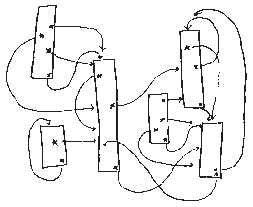
\includegraphics[width=\textwidth]{hypertext.pdf}
	\caption[A Hypertext system]{A hypertext system, from \citeauthor{nelson_computer_1974} (\citeyear{nelson_computer_1974}, p.~\smallcaps{dm47}).}
	\label{fig:hypertext}
\end{marginfigure}

In past decades, the many new properties of \ict s have been recognized and made use of, thus generated new form of culture, new life style, and ``new way of doing politics'' \citep[p.~198]{juris_new_2005}. In his research of anti-corporate globalization activists, \citeauthor{juris_new_2005} found that facilitated by several features of Internet, such as long-distance coordination, horizontal collaboration, highly flexible and decentralized network forms, activists developed their new, and more efficient way of practice, they can reach thousands of activists immediately and easily collaborate between different countries. It has been argued that the Internet and \ict s has faded the borders of time and distance \citep{juris_new_2005,harlow_collective_2012}, that information on the internet could be accessed by all the user almost equally: ``the geographical proximity and content availability are independent of each other'', information could be copied almost immediately and freely \citep[p.~179]{boyle_foucault_1997}, old information is equally easy to access as new ones, neither be worn or damaged through time. The emergence of technologies, especially \ict s, revolutionarily accelerated the process of globalization while the decentralized structure of the Internet removed the local dependency on other methods of exchanging information, thereby creating an alternative global discourse and understanding \citep{chadwick_internet_2006,dencik_alternative_2013}. \marginnote{``We now have the capacity to find common ground with people we will never meet but who we will meet through the Iinternet and through all the modern means of communication[\ldots]''\\\noindent(\citealp{brown_wiring_2009}, \citealp[cited in][p.~1219]{dencik_alternative_2013})} \citet[p.~205]{juris_new_2005} also notes that the virtual space ``can be incorporated into more everyday forms of social, economic, and political life''. Activists in Barcelona use Internet-based collaborative software to ``collectively produce documents regarding real-world initiatives'', they achieved the project smoothly in the intertwined virtual and physical space. It could be argued that the virtual space here is complementary to physical space, and through which the same purpose and practice could be conducted as in the physical space.

However,\marginnote{``[L]aw is a command backed by threats, issued by a sovereign who acknowledges no superior, directed to a geographically defined population which renders that sovereign habitual obedience.''\\\noindent(\citealp{austin_province_1954}, cited in \citealp{boyle_foucault_1997})} it should be noted that the Internet did not become a utopia. \citet{curran_why_2012} argues that the central weakness of the theorising around the Internet is that they mostly focused on the technology while the limits of social context is neglected. Many fantasies created by the advantage of \ict s including Internet technologies such as synchronicity and overcoming the physical distance is only based on the fact that the technology itself is fully accessible, in fact the availability of technology is tightly bound to the political and economical environment of users, which highly depends on actual location of the users. The Internet did bring new possibilities of communication, but only for those places that could afford its infrastructure and willing to embrace it. There is still a huge portion of population with no access to the Internet (see figure \vref{fig:internetpopulation}), while some countries ban or restrict the access to the Internet, such as the Great Firewall of China i.e.\ the \gfw. \citeauthor{curran_misunderstanding_2012} (\citeyear{curran_misunderstanding_2012}, cited in \citealp{dencik_alternative_2013}) lists several limitations of Internet regarding the discourse of globalization, including:%
\begin{figure*}[!htbp]
	\centering
	\includegraphics[width=\textwidth]{InternetPopulation.png}
	\caption[Internet population and penetration based on 2011 data]{Internet population and penetration based on 2011 data, this map illustrates the total number of Internet users in a country as well as the percentage of the population that has Internet access, from \citet{graham_internet_2013}.}
	\label{fig:internetpopulation}
\end{figure*}
\begin{enumerate}
	\item the world is very unequal and this limits participation in an internet-mediated global dialogue;
	\item the world is divided by language and only 15\% of the population understands English;
	\item language is a medium of power so those writing or speaking in English will reach a much larger public than those conversing in, say, Arabic;
	\item the world is divided by bitter conflicts of value, belief and interest;
	\item nationalist cultures are strongly embedded in most societies;
	\item authoritarian governments have developed ways of managing the net and of intimidating would-be critics;
	\item inequalities within countries – not just between them – can distort online dialogue.
\end{enumerate}
The differences in language, culture, and value actually become the border and distance in the virtual space. In the research conducted by \citet{dencik_alternative_2013}, the author detailed the efforts of website OhmyNews, the very successful citizen reporter platform expanded itself to the global scale in 2004, opening its English version OhmyNews International. According to the founder \citet{oh_end_2004},```Every Citizen is a Reporter' has been applied only to Korean speakers. Now it will grow to include people everywhere''. However, the attempt failed, OhmyNews International stopped its citizen journalism feature in 2010, due to limits of funding and difficulties of handling stories from worldwide. It is pointed out that in 2009--2010 in content produced in the site, Europe and North America took the largest share, and only 4\% of which is about Africa. The principle of ``Every citizen is a reporter'' actually resulted in those those who were from most powerful countries, who have better access to the Internet, better English skill, would have most voice, even on the Internet. \citet{dencik_media_2011} argues that the transformative potential in the virtual space as political space, rather than necessarily challenging the dominant power structure, could actually replicating it, or even legitimizing it.

\section{Summary}

To summarize, this chapter explored the idea of conversion between everyday and political expressions, and the relation between physical and virtual spaces. As the term \textit{politics} could be defined as the activities that challenge or maintain the established order, when lacking power or resources for direct defiance to the power holders, the political expression of subordinate classes would transform from explicit action or discourse to implicit ones. Through the creative use of public space, which has been usually designed with clear purpose, the practice of everyday life from subordinate people could blurs the discipline created by the authorities, and create contested insurgence space that claims their own demand.

Based on Mcluhan's theory of medium as extension of human, this chapter also reviewed the idea that the virtual space i.e.\ the metaphorical space created by \ict s as an extension of the physical urban space. On one hand, the nature of the virtual space can break certain borders in the physical space, and thus accelerate or even initiate new social communication and activity; on the other hand, due to the complex reality of imbalanced distribution of Internet infrastructure, language, and other social economical factors, the power relations and politics appear in the physical world have often been extended into the virtual space, that the virtual space sometimes does not fix the power difference, but continues it, or even amplifies it.

\begin{figure}[!htbp]
	\centering
	\begin{tikzpicture}[x=1.3in, y=1.3in, font=\footnotesize]
	\draw[very thick] (1,1) circle [radius=.1];
    \draw[very thick] (1,2) circle [radius=.1];
    \draw[very thick] (3,1) circle [radius=.1];
    \draw[very thick] (3,2) circle [radius=.1];

    \draw [<->] (1,1.15) -- (1,1.85);
    \draw [<->] (3,1.15) -- (3,1.85);
    \draw [<->] (1.15,2) -- (2.85,2);
    \draw [<->] (1.15,1) -- (2.85,1);

    \draw (1,0.85) -- (1,0.65) node [below] {ordinary};
    \draw (3,0.85) -- (3,0.65) node [below] {political};
    \draw (0.85,1) -- (0.65,1) node [left] {virtual space};
    \draw (0.85,2) -- (0.65,2) node [left] {physical space};

    \draw [<->] (1.15,1.15) -- (2.85,1.85);
    \draw [<->] (1.15,1.85) -- (2.85,1.15);

    \node [rectangle, fill=white] at (2, 1.5) {power relations};
\end{tikzpicture}


	\caption[A summary of the theoretical framework]{A summary of the theoretical framework.}
	\label{fig:theo}
\end{figure}

\chapter[\Moha, a Silent Protest Behind the Viral Internet Meme]{{\sc M\'o-h\'a}, a Silent Protest Behind the Viral Internet Meme}\label{case}

\section{The culture background before the early age of Chinese digital era}
\dcap{A}{t the} National Conference of Publicity Ministers held on 10th January 2001, the then-president of the People's Republic of China (\prc) and General secretary of the Communist Party of China (\cpc) Jiang Zemin gave a speech, emphasizing that
\begin{quote}
	The publicity on the Internet should be paid particular attention, we should actively develop, sufficiently use, carefully manage the Internet publicity, make good use of its advantage and avoid its disadvantage, strengthen the impact and ``fighting capacity'' of the Internet publicity, make it a new battle field of political and ideological work\footnote{``Ideological work'' is a political term that commonly used in China, refer to activities and education that on behalf of certain social class or political groups, in order to achieve certain political objective, exerting ideological influence on people, and guide people's behavior on purpose. The term is likely translated from Russian word {\selectlanguage{russian}идеологическая работа} from the Soviet Union \citep{__2008-1}.} and a new medium of international publicity\footnote{Translated from Chinese by the author.}. \citep{__2001}
\end{quote}

As the so called core of the third generation of Chinese leadership, Jiang was facing a totally different picture of the country compared to his predecessors. He was nominated as the president unexpectedly in 1989, after the largest political protest referred as '89 Democracy Movement, including the 1989 Tiananmen Square protests and series of protest and demonstration through the country appealing for liberalization, freedom of the press, and re-evaluate the recently dead former president Hu Yaobang who was blamed within the \cpc\ for encouraging democracy and freedom, to replace his predecessor Zhao Ziyang, who was purged for his sympathize attitude to protesters. During the movement, Jiang as the then-mayor of Shanghai, successfully put down the protest by 1.\ appeasing protesters by direct informal communicate;\marginnote{See appendix \vref{timeline} for a more detailed timeline.} 2.\ employing police to guard main streets, ensure the order of regular operation of the city not affected; 3.\ putting pressure on the publisher of the newspaper \textit{World Economic Herald}, which published article supporting the movement and criticized the attitude of government \citep{kuhn_man_2005}.

Jiang's reaction to the protest to an extent represent his political position in his entire career, and a series of policies initiated during his presidency that influence the development direction of the country. One major reason of the '89 Democracy Movement is the Economic Reform initiated by Deng Xiaoping that introduced market economy, privatization, and foreign trade. The policy not only brought in western commodities, but also culture, knowledge, and here more important, political ideologies. Figure \ref{fig:westbook} shows the amounts of published philosophy literatures between 1980--1989, it is clear that the number was increasing and reached its peak at late 1987, then dropped to a very low point in 1989, i.e.\ when the '89 Democracy Movement occurred. Many publishing houses, especially university presses were formed the catastrophe of the Cultural Revolution and the launch of Economic Reform policy. In the period the western theories of democracy and freedom were extremely attractive for people in China, and apparently were learnt with passion \citep{__2011}.
\begin{figure}[!htbp]
	\centering
	\begin{tikzpicture}
  \begin{axis}[
  ybar,
  ymin=0,
  ymax=70,
  width=\textwidth,
  height=3in,
  grid=both,
  label style={font=\footnotesize},
  ytick distance=10,
  xtick distance=1,
  x tick label style={/pgf/number format/.cd, fixed,precision=0, set thousands separator={}},
  xlabel=year,
  ylabel=amount]
    \addplot[black,fill=white] table [x=year, y=amount, col sep=comma] {data/westbook.csv};
  \end{axis}
\end{tikzpicture}

	\caption[Amounts of translated western philosophy literatures, 1980--1989]{Amounts of translated western philosophy literatures, 1980--1989, reproduced from \citet{__2011}.}
	\label{fig:westbook}
\end{figure}

Except of the experience of ``fixing'' the citizens demonstration, Jiang also have a rich overseas study background---he used to work and study in Russian and Romania, and always keen to learn foreign languages. He was familiar with western context and its politics, however he used these knowledge in his own ways: on one hand, he catched the world's background of economic growth and promoted market economy, achieved a rapid economical development in China during his tenure, on the other hand, based on his knowledge of domestic and overseas citizen political activities, he introduced a series of policies to avoid all the ``unstable''  factors, and to make use of media, culture, and education to consolidate the domination of the government and authorites and to conduct their policies \citep{kuhn_man_2005,__2004}.

\section{The Internet censorship and the Great Firewall}

As \marginnote{{\tt "Ueber die Grosse Mauer erreichen wir alle Ecken der Welt"}\\\noindent{\tt "Across the Great Wall we can reach every corner in the world"}\\\noindent\citep{wang_first_1987}}a new and powerful media, Internet drew the attention of the government soon after it went popular. The first use of Internet in China can be tracked back to 1987 \citep{wang_first_1987,shrum_origin_2007}. In 1994, after test and building of infrastructure, China has been officially recognized able to access to Internet. In 1996, the China Golden Bridge Network opened a circuit to the \smallcaps{USA}, and started to provide service to individuals \citep{cernic_evolution_2001}.
\begin{figure*}[!htbp]
	\centering
	\begin{tikzpicture}[baseline]
  \begin{axis}[
  ymin=0,
  xmin=1997,
  xmax=2016,
  width=.6\textwidth,
  height=3in,
  yticklabel pos=upper,
  ytick distance=500,
  grid=both,
  label style={font=\footnotesize},
  x tick label style={/pgf/number format/.cd, fixed,precision=0, set thousands separator={}},
  legend style={legend pos=north west,font=\footnotesize},
  legend cell align=left,
  xlabel=year,
  ylabel=number of Internet users (millions)]
    \addplot[color=black, mark=square] table [x=year, y=china, col sep=comma] {data/internetuse.csv};\addlegendentry{China}
    \addplot[color=black, mark=triangle] table [x=year, y=world, col sep=comma] {data/internetuse.csv};\addlegendentry{worldwide}
  \end{axis}
\end{tikzpicture}
\begin{tikzpicture}[baseline]
  \begin{axis}[
  ymin=0,
  xmin=1997,
  xmax=2005,
  width=.4\textwidth,
  height=3in,
  yticklabel style={
        /pgf/number format/fixed,
        /pgf/number format/precision=5},
  %ytick distance=500,
  grid=both,
  label style={font=\footnotesize},
  x tick label style={/pgf/number format/.cd, fixed,precision=0, set thousands separator={}},
  legend style={legend pos=north west,font=\footnotesize},
  legend cell align=left,]
    \addplot[color=black, mark=square] table [x=year, y=china, col sep=comma] {data/internetuse.csv};\addlegendentry{China (zoomed in)}
    %\addplot[color=black, mark=triangle] table [x=year, y=world, col sep=comma] {data/internetuse.csv};\addlegendentry{worldwide}
  \end{axis}
\end{tikzpicture}


	\caption[Numbers of Internet users in China, 1997-2016]{Numbers of Internet users in China and worldwide, 1997-2016, Source: \citet{cnnic__2016}, and \citet{internet_live_stats_internet_2016}, which was estimated based on the data from International Telecommunication Union, World Bank, and United Nations Population Division.}
	\label{fig:internetchina}
\end{figure*}
After the introduction of Internet, the population of Internet users experienced a rapid increase, along with the global trend, until 2000 it doubled each year (see figure \vref{fig:internetchina}), and reached 53.2\% of the national total population at the end of 2016 \citep{cnnic__2016}.

The state's realization of supervising the information on the Internet was prompt. In 1996, the Ministry of Posts and Telecommunications (\mpt)\footnote{The predecessor of the current Ministry of Industry and Information Technology (\miit).} issued the \textit{Regulations of China on Administration of the Chinese Public Internet Connection to the International network}\footnote{\citet{__1996}, title and quotation translated by the author.}, mentioned that:
\begin{quote}
	\begin{description}[font=\rm]
		\item[\smallcaps{article 10}] Any organization by the author or individual must not use Internet to engage in criminal activity that harm national security or cause leak of state secret; must not use the international network to read, copy, produce, or spread information that harm national security, disorder the social order, or is obscene or pornographc.
		\item[\smallcaps{article 12}] Any individual or organizational Internet user, or Internet service provider must cooperate with relevant national department to supervise and examine the information security of international network, and provide material and convenience when necessary.
	\end{description}
\end{quote}
It is worth noting that, from this very early point, the \mpt\ already started to emphasize its right to collect information from Internet users and Internet service provider (\isp), and make distinction between domestic network and ``international network''.

Early in 1996,\marginnote{``While American and European governments have to legislate themselves the power to control the Internet, this is the default position for the Chinese government, and therefore constitutes one of the defining features of online China. The Internet, and by extension online China, are `government allowed'.''\\\noindent\citep{herold_noise_2011}}\ according to \citet{barme_great_1997}, the Public Security Bureau (\psb) already started to log the personal information of Internet users and filter the ``harmful'' websites by both administrative and technical means: individuals applying for Internet access have to provide \smallcaps{id}s, personal information including address, work place etc., and sign the \textit{Net Access Responsibility Agreement} which includes an agreement to not ``read, copy, produce, or spread information that harm national security, disorder the social order, or is obscene or pornographic''; and \isp s had been running keywords-based filtering to block websites that contain political sensitive materials, which is relatively easy since all international connections have to be made through state owned \isp s, and the access routes are owned and controlled by the government, from which individuals and organizations only have the right to rent bandwidth.  \citep{herold_escaping_2012,herold_noise_2011,barme_great_1997}. A study conducted by \citet{zhang_behind_2006} directly with the policy makers shows that the new technologies not only caused new policies and ``game plan'', but also reshuffled of policy making process, the ``frame of negotiation'' \citep[p.~147]{price_media_2002}. The main responsibility of managing the media and information had been shifted from directly the \cpc, to the committee China Internet Network Information Center (\cnnic) Steering Committee formed in 1997, which consisted of both scholars and government officers \citep[p.~281]{zhang_behind_2006}. The interviewed authorities states the ``two-hand strategy'' of policy making, that ``promoting development of the [I]nternet, [policy makers] have to supervise and regulate the content'', the government was intended to make use of the benefit of economical growth and information exchange by encouraging it, but meanwhile keep away the unfavorable materials \citep{zhang_behind_2006}.

The major instrument that the Chinese government currently use, the \gfw\footnote{This term was likely be coined by \citet{barme_great_1997} in the \textit{WIRED} magazine article, later was commonly accepted but never be referred nor admitted \textit{per se} by the Chinese official.}, started its development in 1998 (although the term was used \textit{avant la lettre} a year before as a metaphor to the general idea of Chinese Internet censorship), and lunched at 2003 according to the leading designer of the \gfw\ Fang Binxing \citep{global_times_great_2011}. So far, the major techniques of the \gfw\ include \smallcaps{ip} blocking and \smallcaps{dns} tampering and hijacking, which blocks sensitive blacklisted websites e.g.\ Google or specific service on specific servers directly; the deep packet inspection and keyword filtering, which could censor the real time Internet traffic and block the webpage or service that contains specific keyword, and recently even active attack \citep{xu_deconstructing_2016,yuen_becoming_2015,perlroth_chinese_2015}.

However, a more powerful way is the self-censorship, where the ``the general sense that you are under surveillance acts as a disincentive. The key to controlling the Net in China is in managing people, and this is a process that begins the moment you purchase a modem'' \citep{barme_great_1997}. The policy makers see the act of censoring not only as a means of regulation, but a kind of education, through which website managers and users would regulate what they post on the Internet by themselves \citep{zhang_behind_2006}. In 2015, after the code hosting website GitHub have been DDoS attacked likely by Chinese government\footnote{The Ministry of Foreign Affairs of the \prc\ (\mfa) did not admit nor deny the government initiate the attack, however some research shows that the attack has the similar Internet characteristics as the \gfw, therefore it is mostly believed that this is the action of the Chinese government \citep{brandom_last_2015,perlroth_chinese_2015}.}, many Chinese users of GitHub rise the argument that users should regulate themselves not post political sensitive materials on the site, since the government may ban the site for these materials and all ``innocent'' users would be affected \citep{__????-16}. Domain websites in China were asked to sign a pledge in 2002, in which they promised to not produce and spread pernicious information on their website, remove sensitive materials (otherwise relevant staff could face expulsion), and to monitor foreign-based websites \citep{the_guardian_chinese_2002}. The \usa\ Internet company Yahoo! also signed the pledge, and on 2006 it was criticized in west for providing information of online activities of user to the Chinese government, and caused the arrest of a pro-democracy journalist Shi Tao \citep{the_associated_press_yahoo_2007}. The standard of the self-censorship became more strict, in a conference at 2016, the Cyberspace Administration of China (\cac) asked domain websites to verify the body of responsibility for all posted information, control the sources of news posts (commercial websites were no longer allowed to produce news posts by themselves), and be responsible 24$\times$7 in the case of emergency. Earlier this year many originate news sections of major websites were shut down for posting mistaken information related to the president Xi Jinping \citep{_8_2016}.

By conducting the sense of insecurity, through privatized enforcement (letting \isp s to take the responsibility of filtering contents) and surveillance, the state actually make the virtual space a Panopticon, that the exact choice of censored words never been told or explained to the users, but was given the sense that certain content are generally \textit{known} to exist \citep{vuori_lexicon_2015,boyle_foucault_1997}. The research conducted by \citet{vuori_lexicon_2015} concerning keyword filtering systems on Chinese social networks shows that almost 16.26\% of all messages posted on the largest Chinese tweeter-like microblog service Weibo are deleted over time, especially those are ``politically sensitive'' or potentially lead to ``collective action'' one third of censored keywords are related to names of leading members of the \cpc. According to \citet{foucault_security_2007}, through the technique of surveillance and correction, discipline is operated in the way that people do things spontaneously and without knowing the influences on their behaviour. While covered by the means of technologies, the manipulation of information by sovereign is usually accepted by the users as they are without noticing its political origins. The censorship in Chinese Internet is not intended to actually stop people seeing the political related contents, at least the names of party leaders are being repeatedly mentioned on official medias all the time, but to make the free communication about the ``leading personalities'' freely by simply referring their names more difficult, and thus ``hinders their ability to form shared critical opinions on them and their policies'' \citep[p.~413]{vuori_lexicon_2015}.

\section{The viral subculture of toad-worshiping}\label{sec:moha}

If one is using Chinese social networks in recent years, one would occasionally see curated stickers, pictures, videos, and quotes from the ex-president (from 1989 to 2002) Jiang Zemin. The culture phenomena referred as \moha\ (膜蛤, literally toad worship) went increasing popular especially after Xi Jinping became the current president in 2012.
\begin{marginfigure}
	\includegraphics[width=\textwidth]{mohasample1.jpg}
	\caption[A sample of meme picture based on the portrait of Jiang Zemin]{A sample of meme picture based on the portrait of Jiang Zemin.}
	\label{fig:mohasample1}
\end{marginfigure}

In the term ``\moha'', Jiang has been assimilated to a toad (蛤蟆, \textit{h\'a-ma}) for his signature appearance: oversized black frame glasses, broad mouth, and high-waisted pants \citep{_jiang_2016}. The metaphor is first used by Falun Gong (also known as Falun Dafa) as an insulting nickname of Jiang. Falun Gong is a spiritual practice group that has been categorized as ``heretical organization'' by the Chinese government and banned in mainland China since late 1999. The group has held a radical and hostile attitude toward the \cpc\ and the then-party leader Jiang. In early 2000s, around ten years before \moha\ eventually became popular, the Falun Gong created, although it went against their original intention, the basic ground of the subculture, and funded one of the most popular Internet censorship circumvention software at that time, Freegate, that allows Internet users in mainland China to bypass the \gfw\ and accessing the blocked content. Freegate features Epoch Times\footnote[][-.7cm]{The website has been hosted in \usa\ and banned in Chinese Internet since the beginning.} as its homepage. The website contains a lot of information that against \cpc\ and Jiang himself, lots of which are travesty (see figure \vref{fig:flg1}) and crudely made folk stories e.g.\ portraying Jiang as a sprite of toad.
\begin{figure}[!htbp]
	\centering
	\includegraphics[width=\textwidth]{flg1.jpg}
	\caption[A cartoon posted on the Falun Gong sponsored news website Epoch Times]{A cartoon posted on the Falun Gong sponsored news website Epoch Times. Left text: traitor of China/foreign spy/quisling Jiang Zemin; right: accuse Jiang Zemin. Source: \citet{__????-162}.}
	\label{fig:flg1}
\end{figure}
They also posted large amount of video materials related to Jiang, especially those with his negative figures. Most users of Freegate at that time are usually high-educated (accessing most blocked websites requires English reading skill, and basic computer skills) and politically pro-liberalization (bypassing the \gfw\ is politically ``dangerous'' in the context of \cpc\ conservatives). However, these effort Falun Gong made did not make big influence on most Chinese Internet users, even those who bypassed the \gfw: most of them would not believe the exaggerated stories, at most amused by the funny behavior of the president in those materials.

In this phenomena, the funniness of Jiang himself played an important role for its viral spreading. His rich overseas experience, interests in art and foreign languages, and his exhibitionist, humorous nature made his very different figure compared to other political leaders in China. In many of his video footages, mostly available on non-Chinese websites such as YouTube and treated as treasures by toad-worshippers, he plays music, sometimes with local instruments during overseas visit, dances, and sings in public occasions. During his 1993 visit to \usa, he happily invited Bill Clinton to play saxophone with him \citep{kuhn_man_2005}. In his interview with Mike Wallace, he answered Wallace's harsh questions about the accusation of dictatorship and '89 Democracy Movement calmly with smile, sometimes even sidestepping the translator and answering directly in English.

The major materials used to produce the \moha\ related memes, derivative works, and parodies are three videos (will be referred as \smallcaps{video 1}, \smallcaps{2}, and \smallcaps{3} afterward):
\begin{enumerate}
	\item The\marginnote{\smallcaps{video 1} is available at \url{https://youtu.be/NsGbhDVFxQw}} video of Jiang's angry response to Hong Kong journalists \citep{pbs_nc_2000}. In a media session, Jiang was asked whether Beijing would endorse the then-chief executive Tung Chee-hwa for a second term. After which he got angry,  then angrily chastised the journalist for around three minutes \citep{landler_leader_2000}.
	\item The aforementioned\marginnote{\smallcaps{video 2} is available at \url{https://youtu.be/3w4dy-VZjBw}} video of Jiang's interview with Mike \citet{wallace_president_2000}.
	\item The video\marginnote{\smallcaps{video 3} is avaliable at \url {https://youtu.be/lsZjnO4NwYw}} of Jiang's revisit of China United Engineering Corporation on 2009. Jiang used to work in the predecessor of this corporation as a engineer. In the video he summarized his experience of being summoned to Beijing and unexpectedly became the president, and his ``three achievements'' during his term. While receiving a gift given by the staff, he said ``This book you give me\ldots\ \textit{Excited!}\footnote{The word was said in English.}''.
\end{enumerate}
Almost every sentence in \smallcaps{video 1} (a more detailed analyse of the creation of memes out of the video is presented in appendix \vref{script}), many screenshot from \smallcaps{video 2}, and lots of sentence from \smallcaps{video 3} especially a piece of poem Jiang read during his speech and the ``excited!'' he said in English became the most popular quotes in the \moha\ subculture. Figure \vref{fig:keywords} shows the trend of search interest from China. Five keywords are selected:
\begin{figure*}[ht]
	\centering
	\begin{tikzpicture}[baseline]
  \begin{axis}[
  ymin=0,
  xmin=2004-01-01,
  xmax=2017-08-01,
  ymax=100,
  width=\textwidth,
  height=3in,
  grid=both,
  y filter/.expression={y==0 ? nan : y},
  label style={font=\footnotesize},
  x tick label style={rotate=45,/pgf/number format/.cd, fixed,precision=0, set thousands separator={}},
  legend style={legend pos=north west,font=\footnotesize},
  legend cell align=left,
  xlabel=year,
  date coordinates in=x,
  date ZERO=2004-01-01,
  xticklabel=\year.\month,
  ylabel=popularity,
  xtick = {
  {2004-01-01},
  {2004-07-01},
  {2005-01-01},
  {2005-07-01},
  {2006-01-01},
  {2006-07-01},
  {2007-01-01},
  {2007-07-01},
  {2008-01-01},
  {2008-07-01},
  {2009-01-01},
  {2009-07-01},
  {2010-01-01},
  {2010-07-01},
  {2011-01-01},
  {2011-07-01},
  {2012-01-01},
  {2012-07-01},
  {2013-01-01},
  {2013-07-01},
  {2014-01-01},
  {2014-07-01},
  {2015-01-01},
  {2015-07-01},
  {2016-01-01},
  {2016-07-01},
  {2017-01-01},
  {2017-07-01}
  }]
    \addplot[only marks, mark=pentagon] table [x=month, y=popularity, col sep=comma] {data/excited.csv};\addlegendentry{excited}
    \addplot[only marks, mark=diamond] table [x=month, y=popularity, col sep=comma] {data/gouliguo.csv};\addlegendentry{苟利国家生死以}
    \addplot[only marks, mark=o] table [x=month, y=popularity, col sep=comma] {data/hah.csv};\addlegendentry{蛤蛤}
    \addplot[only marks, mark=+] table [x=month, y=popularity, col sep=comma] {data/hkj.csv};\addlegendentry{香港记者}
    \addplot[only marks, mark=x] table [x=month, y=popularity, col sep=comma] {data/tanxiao.csv};\addlegendentry{谈笑风生}
    \addplot[only marks, mark=star] table [x=month, y=popularity, col sep=comma] {data/xum.csv};\addlegendentry{续命}
  \end{axis}
\end{tikzpicture}


	\caption[The search interest over time of \moha\ related keywords from China, from Jan 2014 to Jul 2017]{The search interest over time of \moha\ related keywords from China, from Jan 2014 to Jul 2017. A value of 100 is the peak popularity for the term, and a value of \textit{x} represent the keywords' popularity is \textit{x}\% of its peak value. Source: \citet{google_google_????}. Sudden zero points are considered as error and have been ignored in the plot.}
	\label{fig:keywords}
\end{figure*}
\begin{description}
	\item[Excited] This is the word Jiang said during the visit from \smallcaps{video 3}. It is also one of the most commonly referred word in the \moha\ subculture, it is short, easy to remember and is flexible to be used in varies way. It is noticeable that even \textit{excited} is a common English word that not only used as a meme, its search interest also experienced the similar increase along with the other exclusively \moha\ related keywords.
	\item[苟利国家生死以 (Were it to benefit my country I would lay down my life)] This is the first of two sentence of the poem Jiang recited in \smallcaps{video 3} \footnote{苟利国家生死以,岂因祸福避趋之。(\textit{Were it to benefit my country I would lay down my life; What then is risk to me?}, translation from \citealp{central_compilation__translation_bureau_2015_2015}). It was originally from a poem written in 1842 by Lin Zexu.}. He used this to show his determination when he was nominated to be the president. This represent Jiang's allusive personality, and was also frequently quoted by toad-worshippers, sometimes as it is, sometimes abbreviated form such as using the first character 苟 (\textit{g\v ou}), or initial of both sentence 苟岂 (\textit{g\v ou q\v{\i}}), their homophonies, etc.
	\item[蛤蛤 (h\'a-h\'a, toad)] This is the nickname of Jiang given by toad-worshippers. 蛤 (\textit{h\'a}) Literally means toad or clam, but if used repeatedly as \textit{h\'a-h\'a}, this word can be considered exclusively used by the \moha\ subculture, therefore it is chosen to indicate the popularity of the subculture.
	\item[香港记者 (Hong Kong journalist)] This term is from \smallcaps{video 2}, referred to the Hong Kong journalist who was angrily chastised by Jiang. This term is not only used by toad-worshippers, but also used in in everyday conversation, it could be clearly seen from figure \vref{fig:keywords} that even the term also been used elsewhere, its search interest still increased significantly after 2014.
	\item[谈笑风生 (talk cheerfully and smoothly)] This is an idiom Jiang used in \smallcaps{video 1} to referred to his interview with Mike Wallace.
	\begin{marginfigure}
		\begin{tikzpicture}[baseline]
  \begin{axis}[
  ymin=0,
  xmin=2013-01-01,
  xmax=2017-08-01,
  ymax=100,
  width=\textwidth,
  height=2in,
  grid=both,
  y filter/.expression={y==0 ? nan : y},
  label style={font=\footnotesize},
  x tick label style={rotate=45,/pgf/number format/.cd, fixed,precision=0, set thousands separator={}},
  legend style={legend pos=north west,font=\footnotesize},
  legend cell align=left,
  xlabel=year,
  date coordinates in=x,
  date ZERO=2004-01-01,
  xticklabel=\year.\month,
  ylabel=popularity,
  xtick = {
  {2013-01-01},
  {2013-07-01},
  {2014-01-01},
  {2014-07-01},
  {2015-01-01},
  {2015-07-01},
  {2016-01-01},
  {2016-07-01},
  {2017-01-01},
  {2017-07-01}
  }]
    \addplot[color=black, mark=star] table [x=month, y=popularity, col sep=comma] {data/xum.csv};\addlegendentry{续命}
  \end{axis}
\end{tikzpicture}


		\caption[The search interest over time of the keyword ``续命'' around Aug 2015]{The search interest over time of the keyword ``续命'' around Aug 2015. Source: \citet{google_google_????}. Sudden zero points are considered as error and have been ignored in the plot.}
		\label{fig:keywordsz}
	\end{marginfigure}
	\item[续命 (life extension)] This is a term used frequently in the \moha\ subculture, suggesting that every time someone posts, acts, or reacts at something related to Jiang or relevant memes, Jiang's life would be extended for one second, and eventually would make him immortal. The origin of this action was is likely based on the 2011 news that mistakenly reported Jiang had died \citep{blanchard_china_2011,bbc_hong_2011}, and some similar rumors occasionally popped up afterward. Some toad-worshippers would post ``+1s'' or similar phrases when they see some \moha\ related or triggered content, acknowledging that his life has been extended. Figure \vref{fig:keywordsz} shows a rapid growth of the activity of this term around 17th Aug, which is Jiang's birthday, this was a recent climax of toad-worshippers' activity.
\end{description}

\section{How implicit political expression hijack the ordinary language in the virtual space}
why are there an increasing number of people looking to extend an ex-president's life (even mockingly)? Why there were so many people exchanging gossip of a 90 years old politician, and calling themselves worshipper? Why those materials spread by Falun Gong to bring shame on Jiang, seemingly conversely draw people's affection? \citet[pp.~7--8]{shifman_introduction_2014} states that Internet memes can be defined as ``a \textit{group of digital items sharing common characteristics}\footnote{Emphasised as the original.} of content, form and/or stance'', that ``were created with awareness of each other'' and could be circulated and reproduced through Internet users.

As discussed in section \ref{sec:moha}, the subculture of \moha\ experienced a rapid expansion since 2014, before which almost all the materials of the related memes had already been circulated on the Internet for more than 10 years. As the memes use discourse as material that reflect the socioeconomic factors on communication, and ``only memes suited to their sociocultural environment spread successfully'' \citep{shifman_telegraphic_2014,johnson_mapping_2007}, the reason of the emerging of \moha\ subculture clearly have some relation with the sociocultural environment around 2014. Although Chinese government has taken a series of actions to implement the Internet censorship and surveillance, however in 2000s, it was relatively easy to bypass them by simply install softwares or using \vpn. The current president Xi Jinping came to power at 2012, since then the government has been formulating much tighter policies of culture and personal expressions. According to a 2013 regulation about real-name telephone system approved by \citet{miit__2013}, anyone in mainland China purchasing a mobile phone number have to provide a valid \smallcaps{id}s\footnote[][-2,5cm]{Compared with most western countries, although there are also certain kind of censoring, it is still easy to purchase anonymous mobile phone numbers that able to access to Internet, or hide the user identity (at least on the personal level) using services such as \vpn, Tor, etc. without trouble.}, and another regulation passed in 2015, stipulates that all \isp s should follow the principle of ``real-name in the background, optional in the foreground'' \citep{miit__2015}. Currently most mainstream Chinese \isp s require a valid mobile phone number to register, which means anyone living in China who post unfavoured content on the Internet could be trancked directly to the person. A proxy software developer, who has posted supportive opinion to the Occupy Central campaign\footnote{The campaign took place in Hong Kong, intended to protest to the \prc\ government to grant to the right for universal suffrage for Hong Kong citizens \citep{branigan_occupy_2014}. This campaign was recognized as an illegal Hong Kong independence activity and be denounce by the \prc\ and \cpc\ official \citep{_--_2014}.} on Twitter was arrested in 2014 for Crime of Picking Quarrels \& Provoking Troubles \citep{__????-17}. The first Law specifically about Internet \textit{Cybersecurity Law of the \prc} was passed in 2015, explicitly states that all \isp s must require users to provide their valid \smallcaps{id} when providing Internet accessing service, must cooperate with national security departments when necessary, must report to the national security departments when any illegal information was detected, and could cut down the Internet in certain area when urgent situation appears \citep{__waf}.

The discontent sentiment for Xi's restrictive attitude toward the Internet freedom is another major element in the \moha\ related memes. Figure \vref{fig:jiangxi} shows a pair of book covers of Jiang and Xi's biographies. The former is the actual cover of the book by \citet{kuhn_man_2005}, which takes a positive comment to Jiang's presidency, and has been banteringly praised within the toad-worshippers' group, while the latter is a fictive book cover that has been circulated on the Internet.
\begin{figure}[!htbp]
	\centering
	\includegraphics[width=.45\textwidth]{jiang.jpg}
	\hfill\includegraphics[width=.45\textwidth]{xi.jpg}
	\caption[Satiric fictive book cover of Xi Jinping's biography compared to the actual Jiang's]{Satiric fictive book cover of Xi Jinping's biography compared to the actual Jiang's. Left text: He changed China---A biography of Jiang Zemin; right: He then changed it back---A biography of Xi Jinping.}
	\label{fig:jiangxi}
\end{figure}
While the title of Jiang's biography \textit{The man who changed China} usually be understood as his positive impact on Chinese economic growth, and facilitate formal and informal international communication based on the economic reform policy initiated by Deng Xiaoping. The satiric title \textit{The man who changed China back} implies the unsatisfactory to Xi's policies of strengthen Internet and press censorship and the personality cult built by propaganda \citep{beech_chinas_2016}, and his changing to society back to the ``old society'', which in Chinese context often means feudal, totalitarian imperial society before the mid 20th century \citep{cohen_cultural_1993}. Ironically, both of the pictures were banned in the dominating\footnote{More than two thirds of handset owners use it regularly in 2017 \citep{mcnair_wechat_2017}.} Chinese instant message application WeChat, which displayed as sent in the sender's side but won't be received\footnote{Tested by the author on 3rd July 2017.}. In mid 2017, the cartoon character Winnie-the-Pooh was censored in Chinese social networks because its similar appearance to Xi \citep[see figure \vref{fig:winnie}]{hernandez_winnie--pooh_2017}.

Along with the increasing censorship since 2012, while \textit{talking about politics} or even simply party leaders has been becoming dangerous, people started to search for new way of political expressions. \citet{scott_behind_1990} describes the mechanism of ``public transcripts'' that happens in the public domains that subordinates (or those take the weak side of the power relationship) act with subordination to the dominant power, ``offer a performance of deference and consent while attempting to discern, to read, the real intentions and mood of the potentially threatening powerholder''. However the implied intention that challenging the powerholders, with the coded information that only who with awareness or certain political position can understand, a kind of \textit{unobtrusive dissent} \citep{perry_studying_2007,esarey_political_2008,scott_behind_1990}. In the early 2000s, the materials released by Falun Gong were all explicitly pointed to Jiang himself, with his name and figures. Today, the terms and figures used by toad-worshippers are degraded more and more close to ordinary languages. ``苟'' (\textit{g\v ou}) is a common Chinese characters and usually means nothing if used by its own, however it became a kind of secret signal between toad-worshippers, when someone see an Jiang related content, or simply just want to draw attention of other toad-worshippers, he/she could just post this one single character and noticed toad-worshippers would follow and reply with other characters from the poem.
\begin{marginfigure}[-12cm]
	\includegraphics[width=\textwidth]{pooh.jpg}
	\caption[The picture that has been circulated on the Internet showing Xi Jinping and Barack Obama resemblance to Winnie-the-Pooh and Tigger]{The picture that has been circulated on the Internet showing Xi Jinping and Barack Obama resemblance to Winnie-the-Pooh and Tigger.
		\label{fig:winnie}}
\end{marginfigure}

\begin{figure}[!htbp]
	\centering
	\includegraphics[width=\textwidth]{zhihu.pdf}
	\caption[An answer posted on Chinese question-and-answer website Zhihu implies script of the conversation in the video of Jiang Zemin angrily chastised the Hong Kong journalist]{An answer posted on Chinese question-and-answer website Zhihu implies script of the conversation in the video of Jiang Zemin angrily chastised the Hong Kong journalist, answering the question ``What story could you write if only using punctuation marks?''. Source: \url{https://www.zhihu.com/question/60370256}.}
	\label{fig:zhihu}
\end{figure}

Figure \vref{fig:zhihu} shows a typical implied \moha\ activity, that one of the users of the question-and-answer website Zhihu posted a long list of seemingly meaningless dashes and punctuation marks. They are actually the script from the conversation between Jiang Zemin and the Hong Kong journalist in \smallcaps{video 1}, with all texts been substituted by dashes.
\begin{figure}[!htbp]
	\centering
	\includegraphics[width=\textwidth]{scnst.png}
	\caption[A screenshot from a Chinese bullet comment video website while audience posting ``life extension'' comments]{A screenshot from a Chinese bullet comment video website while audience posting ``life extension'' comments. Source: \url{https://bangumi.bilibili.com/anime/5788/play\# 101771}; The video: \citet{yoshinari_blue_2017}.}
	\label{fig:xmn}
\end{figure}
Figure \vref{fig:xmn} is another example, in a bullet comment video website Bilibili, when the line in the anime mentioned ``九长者'' (nine elders), audiences started posting comment such as ``+1s'' or ``+9s'' on the screen. ``Elder'' is the what Jiang had called himself during his chastise to the journalist: ``today I am not as a president, but an elder, to teach you some experience of life''. The content of the anime does not have any relation to Jiang, and the word has just been used normally, but the toad-worshippers were still be triggered, and hijacked the unrelated material as their own. To an extent, any language, images, or objects that contains or has any similarity to
\begin{enumerate*}
	\item quotes from Jiang, or any homophony of it, e.g.\ ``excited'', ``na\" ive'', etc.;
	\item Jiang's appearance: high waist pants, black frame glasses, or anything looks like them;
	\item any person or action that related to or had been mentioned by Jiang, e.g.\ Hong Kong journalists, ``running fast'', the university Jiang used to studied in (Shanghai Jiao Tong University), etc.;
	\item Any language or object that could be related to the \moha\ subculture itself, e.g.\ anything contains character ``膜'' (\textit{m\'o}: worship/ film/membrane), ``蛤'' (\textit{h\'a}: toad/frog/calm), ``extend'', ``one second'', etc.
\end{enumerate*}
\begin{marginfigure}
	\includegraphics[width=\textwidth]{blm.jpeg}
	\caption[A sketch circulated on the Internet that implies Jiang by glasses and nostrils]{A sketch circulated on the Internet that implies Jiang by glasses and nostrils.}
	\label{fig:simplemo}
\end{marginfigure}

These actions, rather than expressing certain political opinion, is more like a kind of ritual. It is easy to remember and repeat, and is interesting and fun. Every time the \moha\ activity is triggered, whether intentional or by unrelated thing, a context is created that only those who share the knowledge of this subculture---not only know about Jiang, but know him in the way of \moha. Like the Soviet joke describe:
\begin{quote}
	A man is distributing leaflets in Red Square. He is stopped by a policeman, who confiscates them, only to discover that they are blank. ``What are you spreading? They are blank. Nothing is written!'' the surprised guardian of order exclaims. ``Why write?'' is the answer. ``Everybody knows\ldots'' \citep[p.~2]{przeworski_prologue_1991}
\end{quote}
Through the practice of these activities, a counter-discourse was built: \textit{talking about politics} is political, and being political itself is conceived as dangerous in contemporary China. By practicing \moha, toad-worshippers are talking (satirizing, making fun of) about the former top party leader, in a way that their the political critiques have been normalized to a extremely ordinary level that can hardly be censored, censoring single characters is nearly impossible, neither censoring everything with two ovals and two dots (see figure \vref{fig:simplemo}), or simply some dashes (figure \vref{fig:zhihu}). The ritual is a \textit{confirmation} between toad-worshippers. The joke of ``life extension'' could be seen as a calling, that what toad-worshippers actually want to extend is the time with loose policies for speech and political expressions, international communications, and rapid economic growth; and what Jiang's personal figure represents---art lover, can speak many foreign languages, humour (which has  extincted on the two successors of Jiang), and human emotions---he was a president that would chastise a journalist. By contrast, Xi Jinping has been criticized for his bad personal taste: in a speech given in 2014, he listed 112 artists by name without in one time without any detail and context \citep{__2015-3,chin_year_2015}. He also said on another conference that architects should avoid ``strange-looking buildings'' and encouraging patriotic art \citep{alyssa_abkowitz_xi_2014}. It is ironic that although the \gfw\ was actually initiated during Jiang's presidency, due to the technical resource and government's less knowledge to the Internet, compared with later yeas, the period of early 2000s was still the peirod that Chinese Internet users have most freedom.

\chapter{Conclusion}

\dcap{\textit{M}}{\textit{\'o-h\'a} has been} a unique cultural phenomena, not only in China but in the world. Unlike other Internet memes, the memes about Jiang has an unusually long history that more than 15 years. In early 2000s, the spiritual practice group Falun Gong started to release a large amount of materials of the negative images of the then-president Jiang Zemin. Since the Chinese Internet censorship started from 1990s, most of these materials were blocked for regular Chinese Internet users, and only available from overseas or by using proxy software. However, in early 2010s, while after the presidency of the current president Xi Jinping, these materials were used to create a large amount of memes and derivatives, and circulated on the Internet virally since 2014. At the beginning most participants were high-educated groups or tech savvy groups whom have related knowledge and/or could access to proxy software, but along with the subculture of \moha\ (toad-worship) was initiated and became popular, the phenomena involves people from various social groups.

The cause of the phenomena include many factors. A series of culture and information related policies passed during Xi's presidency emphasize a heavy censorship including real-name system, content filtering, restricting foreign contents, tightening the block of proxy software, etc.\ in the culture and Internet scene. The state has been trying to control the domestic Internet as part of its territory, as well as its geographical land, by making the  metaphorical border in order to control the circulation of information, and using technical means to match the online identity with actual person. The discipline was practiced in a way that its political intentions are covered by the technical details, and can hardly be noticed by regular users. The behaviour of regular Internet users is trained and regulated through minor adjustments, creating a sense of insecurity of talking about dangerous, mostly politically sensitive content, and thus the self-censorship is achieved. These pressing regulation raised provoke sentiments among the Internet users. Due to the heavy censorship for the expression criticizing political subjects (policies, the government or the \cpc\ themselves, etc.), and the increasing cost (economical, technical, and political) to access the uncensored Internet---some people have been arrested by posting content that unfavorable for the government, people started searching for alternative way for their political expression. Toad-worshippers use extremely ordinary languages, seemingly irrelevant quotes, minimalist symbols, and everyday objects which can hardly be censored, to trigger and refer to the materials about Jiang, which shared among participants of the subculture. Consider the virtual space as the public space, \moha\ could be understood as a way of using creative way to \textit{loosen} the space, to challenge the heavily regulated order of the public space and create an insurgent space to claim their own demand. People who share the collective knowledge and political position that giving the ability to understand the memes creates the context of \moha. In this shared ``space'', the original meaning of the everyday languages and symbols are hijacked, and become the signal and material of the ritual that allow subordinate people to challenge the discipline established by the state by simply \textit{talking} about politics---by insinuating, even making fun of the former top party leader.
% While the context of \moha---created by people who share the collective knowledge and political position that can understand the memes---emerges, the original meaning of the everyday languages and symbols are hijacked, and become the signal and material of the ritual that allow subordinate people to challenge the discipline established by the state by simply \textit{talking} about politics---by referring to, even making fun of the former top party leader.

The fever of \moha\ provides a valuable opportunity to unpack the complicated contemporary Chinese informal politics, and then the general mechanism of grassroot political discourse and the generation and circulation of Internet memes. Future studies about this topic could be taken: quantitative data is still lacking in the current research, and depth study about the participants and the socio-cultural effect of this subculture are still needed.





\backmatter

\addcontentsline{toc}{chapter}{Bibliography}
\printbibliography
% \printindex % Print the index at the very end of the document

\renewcommand{\thesection}{\Alph{section}}
\renewcommand{\thefigure}{\Alph{section}.\arabic{figure}}
% % \chapter{Appendixes}
\clearpage
\addcontentsline{toc}{chapter}{Appendices}
\markboth{Appendices}{}
\section{The timeline of major events during the '89 Democracy Movement and Jiang Zemin's nomination of president}\label{timeline}
\begin{description}[align=right]
	\item[15/04] Hu Yaobang's death
	\item[16/04] Students stated protest in Beijing and Shanghai
	\item[24/04]\textit{World Economic Herald} published pro-protest articles
	\item[26/04]\textit{People's Daily} published an editorial defined the student protest as a revolt
    \item[-] Jiang Zemin shut down the editorial department of the Herald
	\item[03/05] Thousand of Shanghai citizens protest for dismiss Jiang's mayor position and recover the Herald
	\item[04/05] 200 thousands of students gathered in Tiananmen Square
	\item[-] Zhao Ziyang made a speech supporting the student protesters
	\item[13/05] More than 500 students went on a hunger strike in Tiananmen Square
	\item[17/05] Millions of citizens protested in Beijing
	\item[19/05] Jiang appeased protesters in Shanghai
	\item[22/05] The army attempted to enter Beijing but stopped by the protesters
    \item[-] Deng Xiaoping nominated Jiang Zemin to be the president in replace of Zhao Ziyang
	\item[01/06] Liu Xiaobo and other three protesters started the second hunger strike
	\item[03/06] The army started to advance on the Tiananmen Square and opened fire on protesters
	\item[04/06] The army arrived and began to seal off the square, in the morning protesters was cleared off the square after negotiation
    \item[24/06] Zhao Ziyang was dismissed from his president position and replaced by Jiang Zemin
\end{description}

\clearpage
\section[An analyze of a raw material for \moha\ related memes]{An analyze of a raw material for {\sc m\'o-h\'a}\ related memes}
\label{script}
This appendix includes the script of the video of Jiang Zemin angrily chastised a Hong Kong journalist i.e.\ \smallcaps{video 1}, transcribed and translated by the author based on the original Chinese subtitle, with minor adjustments. This video is chosen as an example here because it is the best known and most widely used material for creation of memes related to the \moha\ subculture.
\begin{marginfigure}
	\includegraphics[width=\textwidth]{video1.png}
	\caption[A screenshot from \smallcaps{video 1}]{A screenshot from \smallcaps{video 1}. Souce: \url{https://youtu.be/NsGbhDVFxQw}, at 3:25.}
\end{marginfigure}
All phrases underlined in the script are being used for creating memes, some for its content and some for its tone when it was said by Jiang. Phrases that are italicized (for the Chinese part, the Kai-type font is used as equivalent) and marked with ``\cann'' are said in Cantonese. Some phrases is said directly in English, which could be read from the script, are also italicized. \smallcaps{jo} refers to the journalist, and \smallcaps{ji} refers to Jiang Zemin.
\ex[glhangstyle=none, everygla=\rm, exnoformat=X:, exno={\smallcaps{jo}}, belowexskip=0pt]
\begingl
\gla
{江主席,} {你觉得} {董先生} {连任} {好不好呀?}//
\glb
{President Jiang,} {do you think} {Mr.\ Tung} {serving a second term} {is a good idea?}//
\endgl
\xe
\ex[glhangstyle=none, everygla=\rm, exnoformat=X:, exno={\smallcaps{ji}}, belowexskip=0pt, aboveexskip=-.5cm]
\begingl
\gla
{\it \underline{好呀}!\rm \cann} {}//
\glb
{\textit{It is}!} {}//
\endgl
\xe
\ex[glhangstyle=none, everygla=\rm, exnoformat=X:, exno={\smallcaps{jo}}, belowexskip=0pt, aboveexskip=-.5cm]
\begingl
\gla
{} {中央} {也} {支持他吗?}//
\glb
{[Does]} {Beijing (the Cental)} {also} {support this (him)?}//
\endgl
\xe
\ex[glhangstyle=none, everygla=\rm, exnoformat=X:, exno={\smallcaps{ji}}, belowexskip=0pt, aboveexskip=-.5cm]
\begingl
\gla
{当然啦!} {}//
\glb
{Of course!} {}//
\endgl
\xe
\ex[glhangstyle=none, everygla=\rm, exnoformat=X:, exno={\smallcaps{jo}}, belowexskip=0pt, aboveexskip=-.5cm]
\begingl
\gla
{为什么} {那么早就提出?} {是否} {没有} {别的人选?} //
\glb
{Why} {put this forward this early?} {Is it because} {there is no} {other [suitable] candidate?}//
\endgl
\xe
\ex[glhangstyle=none, everygla=\rm, exnoformat=X:, exno={\smallcaps{ji}}, belowexskip=0pt, aboveexskip=-.5cm]
\begingl
\gla
{我} {没有} {时间} {} {跟你们谈。}//
\glb
{I} {don't have} {time} {to} {talk about this with you.}//
\endgl
\xe
\ex[glhangstyle=none, everygla=\rm, exnoformat=X:, exno={\smallcaps{jo}}, belowexskip=0pt, aboveexskip=-.5cm]
\begingl
\gla
{江主席,} {欧盟} {最近} {发表了} {一个} {报告,} {说} {北京} {会透过一些渠道} {去影响} {、} {干预} {香港的法治,} {你对这个看法有什么回应呢?}//
\glb
{President Jiang,} {the \smallcaps{eu}} {recently} {released} {a} {report,} {claiming that} {Beijing} {will use some channel} {to influence} {and} {intervene} {the rule of law in Hong Kong,} {what's your response to this opinion?}//
\endgl
\xe
\ex[glhangstyle=none, everygla=\rm, exnoformat=X:, exno={\smallcaps{ji}}, belowexskip=0pt, aboveexskip=-.5cm]
\begingl
\gla
{没听过} {}//
\glb
{I never heard about that.} {}//
\endgl
\xe
\ex[glhangstyle=none, everygla=\rm, exnoformat=X:, exno={\smallcaps{jo}}, belowexskip=0pt, aboveexskip=-.5cm]
\begingl
\gla
{是} {彭定康说的。}//
\glb
{It is} {Chris Patten[1]'s word.}//
\glft[] [1] Chris Patten was the last British Governor of Hong Kong, one of the \smallcaps{uk}'s two members of the European Commission at the time.//
\endgl
\xe
\ex[glhangstyle=none, everygla=\rm, exnoformat=X:, exno={\smallcaps{ji}}, belowexskip=0pt, aboveexskip=-.5cm]
\begingl
\gla
{你们} {媒体} {千万要} {记着,} {不要} {\underline{「见得风,是得雨」[2]}。} {接到这些} {消息,} {你媒体} {本身也要判断,} {明白我的意思吗?} {假使} {\underline{这些完全无中生有的东西,}} {\underline{你再帮他说一遍,}} {\underline{你等于$\ldots$你也有责任吧?}}//
\glb
{You} {media} {must} {remember,} {don't} {``see wind as rain''.} {When getting these} {news,} {you media} {have to make your own judgement,} {you know what I mean?} {If} {something coming out of thin air,} {you keep repeating it,} {you should also take responsibility for it, don't you?}//
\glft[] [2] This is a Chinese idiom, literally means ``hear the wind and claim there is rain'', used to describe those who easily believe something with only a little evidence or hearsay.//
\endgl
\xe
\ex[glhangstyle=none, everygla=\rm, exnoformat=X:, exno={\smallcaps{jo}}, belowexskip=0pt, aboveexskip=-.5cm]
\begingl
\gla
{现在那么早,} {你们就是说支持} {董先生,} {\underline{会不会给人}} {\underline{一种感觉,}} {\underline{就是内定了、钦点了董先生呢?}}//
\glb
{Now it is still early} {but you already showing support to} {Mr.\ Tung,} {will this give people} {a feeling,} {that Mr.\ Tung is selected by imperial order?}//
\endgl
\xe
\ex[glhangstyle=none, everygla=\rm, exnoformat=X:, exno={\smallcaps{ji}}, belowexskip=0pt, aboveexskip=-.5cm]
\begingl
\gla
{} {\underline{没有任何这个的意思。}} {} {还是按照} {香港的$\ldots$} {\underline{按照基本法}、} {按照选举法---} {去产生} {$\ldots\ldots$}//
\glb
{[I]} {didn't mean that at all.} {[The election]} {will still follow} {Hong Kong's$\ldots$} {Basic Law,} {the Election Law---} {to produce} {(the result$\ldots$)}//
\endgl
\xe
\ex[glhangstyle=none, everygla=\rm, exnoformat=X:, exno={\smallcaps{jo}}, belowexskip=0pt, aboveexskip=-.5cm]
\begingl
\gla
{但是} {你们$\ldots$}//
\glb
{But} {you$\ldots$}//
\endgl
\xe
\ex[glhangstyle=none, everygla=\rm, exnoformat=X:, exno={\smallcaps{ji}}, belowexskip=0pt, aboveexskip=-.5cm]
\begingl
\gla
{刚才你问我啊,} {\underline{我可以}} {\underline{回答你一句}} {\underline{「无可奉告」},} {那你们又不高兴,} {那怎么办?} {我的意思不是} {我是} {钦点} {他当下一任。} {你问我} {支持不支持,} {我是支持的。} {我就明确地给你告诉这一点。} {我觉得} {你们啊$\ldots$} {我感觉} {你们新闻界} {还要学习一个,} {你们} {非常} {熟悉} { 西方的这一套理论。 } {你们毕竟还} {\textit{\underline{too young}},} {明白这意思吧?} {我告诉你们} {\underline{我是身经百战了,}} {\underline{见得多了!}} {\underline{西方的哪一个国家}} {\underline{我没去过?}} {你们要知道,} {\underline{美国的华莱士,}} {\underline{比你们不知道高到哪里去了,}} {\underline{我跟他谈笑风生。}} {所以说媒体啊,} {\underline{还是要提高}} {\underline{自己的知识水平,}} {\textit{\underline{识得唔识得啊}} \cann?} {我也给你们着急啊,} {真的。} {\underline{你们}} {\underline{有}} {\underline{一个}} {\underline{好,}} {\underline{全世界跑到什么地方,}} {\underline{你们比其他的西方记者跑得还快。}} {但是呢,} {问来问去的问题啊,} {都} {\textit{\underline{too simple}},} {\underline{\textit{sometimes na\"{i}ve}!}} {懂了没有啊?}//
\glb
{What you just ask me,} {I could} {just say} {``no comment'',} {but that will then make you unhappy,} {what should I do?} {I didn't mean} {I am} {making an imperial order} {to make him serve another term.} {If you ask me} {support it or not,} {I support it.} {I can tell you this clearly.} {I think} {you$\ldots$} {I think} {you field of journalism} {still have to learn more,} {you are} {very} {familiar with} {western theories,} {but you are still} {\textit{too young},} {you understand?} {I tell you,} {I have experienced many battles,} {I have seen a lot!} {Which western country} {haven't I been?} {You know,} {the Wallace from the \usa,} {he was way better than you,} {and I talked with him cheerfully and smoothly.} {So you media,} {should improve} {your level of knowledge,} {\textit{do you understand}?} {I'm worrying about you,} {really.} {You} {have} {one} {advantage,} {you run all around the world,} {even faster than other western journalists.} {But} {the questions you ask,} {are all} {\textit{too simple},} {\textit{sometimes na\"{i}ve}!} {Do you understand?}//
\endgl
\xe
\ex[glhangstyle=none, everygla=\rm, exnoformat=X:, exno={\smallcaps{jo}}, belowexskip=0pt, aboveexskip=-.5cm]
\begingl
\gla
{但是} {能不能说一下} {为什么} {支持董建华呢?}//
\glb
{But} {can you explain} {why} {you support Tung Chee-hwa?}//
\endgl
\xe
\ex[glhangstyle=none, everygla=\rm, exnoformat=X:, exno={\smallcaps{ji}}, belowexskip=0pt, aboveexskip=-.5cm]
\begingl
\gla
{我很抱歉,} {我今天是\underline{作为一个长者}跟你们讲的。} {我} {不是} {新闻工作者,} {但是} {我} {见得太多了,} {\underline{我}} {\underline{有必要}} {\underline{告诉你们一点}} {\underline{人生的经验。}} {刚才} {我很想啊,} {就是我每一次碰到你们,} {我就讲} {中国} {有一句话叫} {\underline{「闷声大发财」},} {我就} {\underline{什么话也不说。}} {\underline{这}} {\underline{是}} {\underline{最好的!}} {但是} {我想,} {我见到你们这样热情啊,} {一句话不说也不好。} {所以} {你刚才} {一定要---} {\underline{在宣传上将来如果你们报道上有偏差,}} {\underline{你们要负责的。}} {我} {没有说} {要钦定,} {没有任何这个意思。} {但是} {你} {一定要} {问我,} {对董先生支持不支持,} {我们不支持他?} {他} {现在是} {特首,} {我们怎么能不支持} {特首?}//
\glb
{My apology,} {today I'm talking to you as an elder.} {I} {am not} {an journalism practitioner,} {but} {I} {have seen a lot.} {I} {am responsible} {to tell you some} {experiences of life.} {Just now} {I really want to,} {every time I see you,} {I (want to) say} {in China} {we have an old saying,} {``remain silent and make big fortune'',} {I} {don't say anything,} {this} {is} {the best!} {But} {I was thinking,} {you have such an enthusiasm,} {it is not nice if I don't say a word.} {So} {just now you} {insist---} {if there is anything inaccurate in your news report,} {you have to take the responsibility.} {I} {didn't say} {we are making an imperial order,} {not at all.} {But} {if you} {insist to} {ask me,} {if I support Mr.\ Tung or not,} {how could we not support him?} {He} {is the current} {chief executive,} {how could we not support} { the chief executive? }//
\endgl
\xe
\ex[glhangstyle=none, everygla=\rm, exnoformat=X:, exno={\smallcaps{jo}}, belowexskip=0pt, aboveexskip=-.5cm]
\begingl
\gla
{但是} {如果说} {连任呢?}//
\glb
{But} {what if} {serving another term?}//
\endgl
\xe
\ex[glhangstyle=none, everygla=\rm, exnoformat=X:, exno={\smallcaps{ji}}, belowexskip=0pt, aboveexskip=-.5cm]
\begingl
\gla
{连任} {也要} {按照} {香港的法律啊,} {对不对?} {要按照} {香港的$\ldots$} {\underline{当然}} {\underline{我们的决定权}} {\underline{也是}} {\underline{很}} {\underline{重要的。}} {香港特别行政区} {是属于} {中国$\ldots$} {中华人民共和国的中央人民政府啊。} {到那个时候我们会表态的!} {明白我这意思吧?} {\underline{你们啊,}} {\underline{不要想}} {\underline{弄个}} {\underline{大新闻,}} {\underline{说}} {\underline{现在已经钦定了,}} {\underline{再把我批判一番。}} {\underline{你们啊,}} {\underline{\textit{na\"{i}ve}!}} {\underline{\textit{I'm angry}!}} {我跟你讲,} {你们这样子啊,} {是不行的!}//
\glb
{The succession} {will also} {follow} {the laws in Hong Kong,} {won't it?} {Follow} {Hong Kong's$\ldots$} {of course} {our (Beijing's) right of decision} {is also} {very} {important.} {The Hong Kong Special Administrative Region} {belongs to} {China$\ldots$} {the Central People's Government of the People's Republic of China.} {We will make our declaration by then.} {You know what I mean?} {You (media),} {do not try to} {make a} {big news,} {saying something like} {``imperial order'',} {then [use it to] criticize me.} {You,} {\textit{na\"{i}ve}!} {\textit{I'm angry}!} {I tell you,} {acting like this,} {does not work!}//
\endgl
\xe




\end{document}
